\section{Approach}
\label{sec:approach}
\begin{figure*}[htbp]
	\centering
	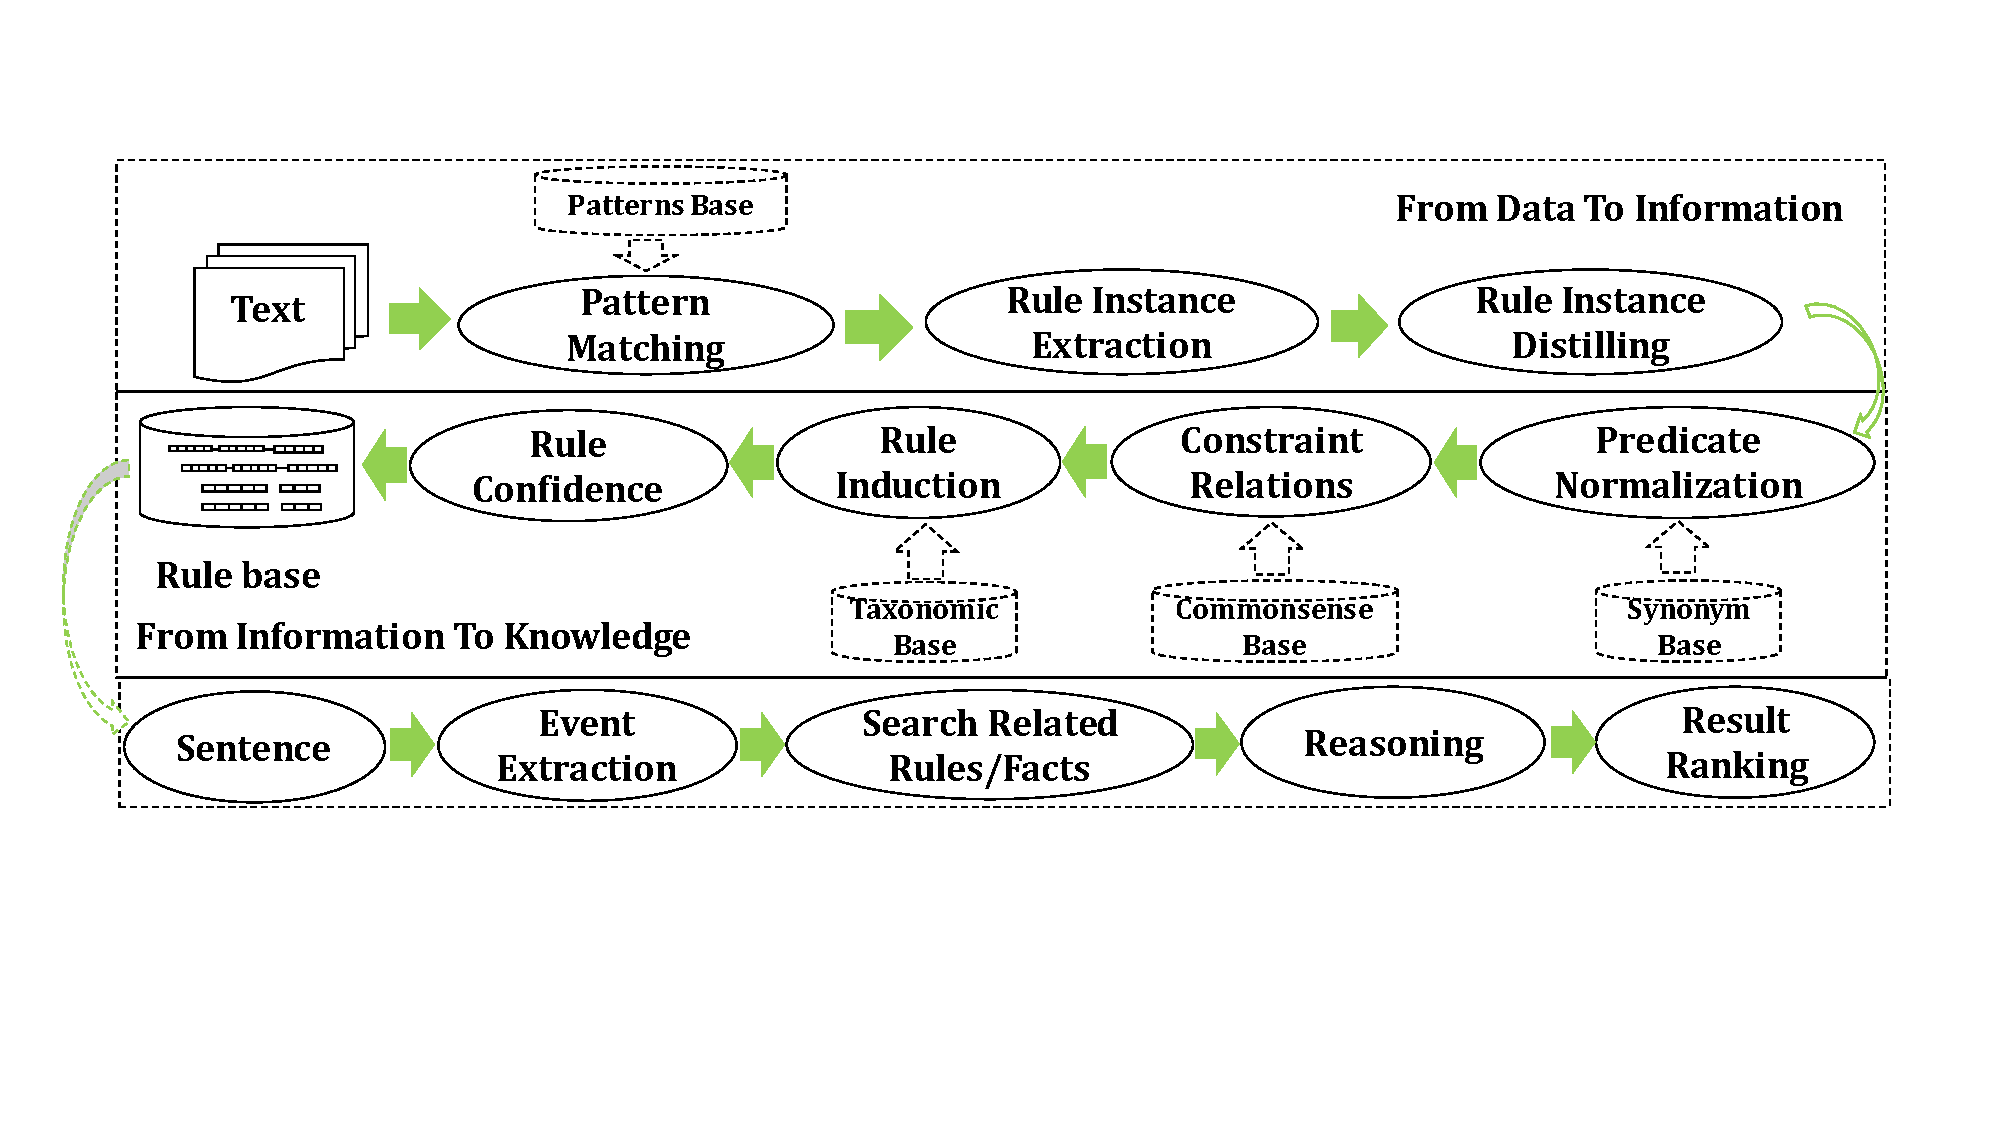
\includegraphics[width=\textwidth]{figures/approach}
%	\caption{Overview of our proposed framework. The top box shows how to extract structured rule instances from large unstructured text. The middle box shows how to exploit external knowledge bases to generalize rule instances into rules. The bottom box shows how to use Prolog to reason with uncertainty on the rules learned.}
	\caption{Overview of the framework. The three parts from top to bottom are rule instance extraction, rule acquisition, and reasoning.}
	\label{fig:approach}
\end{figure*}
In this section, we introduce three parts of our proposed rule learning framework: rule instances extraction, rule acquisition, and causal reasoning, as shown in Figure \ref{fig:approach}.
\subsection{Rule Instance Extraction}
This part is how to extract rule instances from the text.

\textbf{Pattern Matching}
Causality, expressed by natural language texts, can be identified by linguistic patterns known as causal cues \cite{Chang2005}.
We design a set of causal patterns to extract cause span and effect span from the sentences. Causal patterns can be divided into 3 groups based on the pattern structure, shown in Table \ref{tab:pattern_statistics}. The priority of each group represents the order of matching when multiple causal patterns can match a sentence. The stricter the regular expression is, the earlier it matches, and the higher the priority is. In addition, the experiment shows that such kind of patterns can not discover the conjunction of multi-cause events because of people's bad writing habits in the news. 
%\TD{mention conjunction, segment firstly}
%	However, in our experiment, we found that many sentences that matched in the patterns with conjunction are not really conjuncted. \TD{an example}, so we regard them as the normal cause or effect spans.
%
%Alternatively, we can use a more sophisticated way to catch the causality such as \cite{zhao2016event}. In this study, however, we focus more on the precision of causality extraction rather than the recall using more complex patterns, also we think a more sophisticated method used on such noisy text may lead to more errors.
%
%	With these curated patterns, we then use them to match the Chinese \TD{check previous mention about Chinese data} sentences which are segmented firstly to reduce the ambiguity since Chinese has no natural separator. For example,  unsegmented text "由于是" can match both "由于"(cause cue) and "于是"(effect cue). 

%为此###	 短期 来看 , 近期 的 反弹 主要 是 受到 “ 金 九 银 十 ” 传统 消费 旺季 预期 的 影响 , 因为 此时 下游 钢材 市场 出现 回暖 迹象 , 而且 临近 国庆 长假 , 钢厂 有 补库 需求 , 所以 铁矿石 需求 端 得到 支撑 , 目前 主力 合约 的 价格 重回 400 元 / 吨 上方 , 并且 在 节前 曾 最高 上 冲 至 426 元 / 吨 。

%于是### 四川省 食品 发酵 研究所 白酒 专家 余乾伟 告诉 记者 , 茅台酒 由于 是 酱香型 的 发酵 工艺 , 发酵 后 储存 需要 3 年 的 工艺 , 同时 只有 在 茅台镇 茅台 酒厂 所在地 方圆 几 公里 的 地方 才 有 茅台酒 的 酿造 微生物 环境 , 因此 产能 很 难 扩大 , 也 决定 了 茅台酒 资源 的 稀缺性 。

%于是### 对于 是否 可能 导致 “ 囤气 ” 的 行为 , 林 伯 强 认为 可能性 小 , 因为 “ 囤气 ” 成本 较 高 , 且 天然气 占 能源 的 比重 很 小 , 只有 百分之三点几 , 现在 商品 市场 又 很 开放 , 所以 企业 将 成本 转嫁 到 商品 的 可能性 不 大 , 反而 会 促进 企业 节能 减排 。

%	 we use existing dependency parser tool\cite{manning2014stanford} to parse the whole sentence tokens sequence to extract the cause events and effect events to constitute the rule instances.  For cause events, we firstly extract the verbs from the cause tokens span as the predicates. Then extract the subjects and objects of the verbs with the roles of 'nn:subj' and 'nn:dobj' in dependency relations. Lastly, we try to extract the modifiers of these subjects and objects by role of 'nn:compound'. 
%	 After extraction, we can construct many quintuples as cause events with predicate, subject, object and the modifiers of subject and object.	It is the same for effect events. Then we combine these cause events and effect events with a "product" approach to get lots of rule instances. 

%	  Since most sentences have no casual cues and parsing is a very time-consuming operation, we firstly filter out the sentences without casual patterns as a preprocessing.

%	This submodule will be illustrated using the following examples. Consider the following sentence:

%	Feed each sentence into parser tool, then join the  segmented	 output tokens with blanks. For sentence (1), We will get "上 个 月 智利 曾 遭受 8.8 级 大地震 的 袭击 , 导致 铜 价格 上涨 近 6\% 。". Then we exploit the elaborate patterns to match the padded sentence and we can get cause tokens span "上 个 月 智利 曾 遭受 8.8 级 大地震 的 袭击 , " and the effect tokens span "铜 价格 上涨 近 6\% 。".

\textbf{Rule Instance Extraction}
First, we use these causal patterns to extract cause span and effect span. Then, we further extract the cause events and effect events from these two spans via existing dependency parser \cite{Manning}.
The events are mediated by predicates, so we regard each verb in the span as a predicate. Then, find out the subject and object corresponding to each predicate, and get their modifiers. Meanwhile, we also consider the negative dependency of the verb and mark it behind the predicate, which is a practical implement trick. For example, `occur\_1' indicates `occur', while `occur\_0' means `not occur'. 
%These compound nouns are placed at the event as the same order appeared in their origin sentence. 
Since it may be many predicates in each span, which means many events exist in cause span or effect span, we do a Cartesian product of these cause events and effect events as the extracted rule instances. As the comment of philosopher David Hume about causality that the frequency of causal events will be higher than these are non-causal, filtering will alleviate the noisy rule instances. 

%The events in rule instances are mediated by the predicate, namely verb, so we regard each verb in the tokens span as a possible predicate. Then, we find the corresponding subject and object of each predicate. 
%Here, we can get subject and object of each predicate beyond the scope of its corresponding event's tokens span which is an advantage of parsing the whole sentence before matching the cause and effect spans since it can alleviate the parsing error by feeding more context information into the parser.
%Last, we get the modifiers of the subject and object with the dependency relation of 'compound:nn' or 'nmod:assmod', which can be also beyond the scope of its belonging token spans. Meanwhile, we also consider the neg relation of the predicate, we mark it behind predicate, which is a small implement trick. '\_0' means the predicate is negative, while '\_1' means the predicate is positive. 
%These compound nouns are placed at the event as the same order appeared in their origin sentence. 
%Since it may be more than one predicates in cause tokens span or effect tokens span, which means we can get more than one structured events from cause tokens span or effect tokens span, we do a Cartesian product of these cause events and effect events to get more combined rule instances. as the comment of philosopher David Hume about causality, The frequency of causal events will be higher than these are non-causal.  
%We believe that the right rule instances will be appeared more often than the corrupted. 
%Also, later, we will rank the low frequency pairs into the back and filter the undesired rule. From sentence (1), we can get many rule instances, one desired rule instance is ('国际 石油', '价格', '攀高\_1', '', '')$->$('橡胶', '价格', '上升\_1', '', ''). From sentence (2), we can get many rule instances, ('', '乙醇', '增长\_1', '', '')$->$('玉米', '价格', '上涨\_1', '', '') is our desired. Meanwhile we also consider the neg relation of the predicate, we mark it behind predicate, which is a small implement trick. '\_0' means the predicate is negative, while '\_1' means the predicate is positive.

\textbf{Rule Instance Distilling} Some heuristics can discard bad rule instances led by event extraction. For example, a) pronouns appearing in events are meaningless. b) some verbs should not be predicates, such as `say', `state'. c) complete semantic. An event should have at least one subject or object.
% c)the length of each role(subject, object and so on) of the event should be limited because the parser can cause errors.

\subsection{Rule Acquisition}
The part is how to exploit external knowledge bases to generalize rule instances into rules.

\textbf{Predicate Normalization}
Predicates in different words may express the same meaning, such as `raise', `rise', `increase'. We use Ciling\footnote{ \url{ http://www.bigcilin.com/}}, the largest word-level Chinese synonym resource, to normalize the predicates. We ignore verb disambiguation to reduce the complexity of the framework.

%	Then, we would like to generalize these rule instances into candidate rules shown in the Figure \ref{fig:overview}'s middle part. This rule generalization component mainly contains two steps. The first step is predicate generalization and the second step is argument generalization. Predicate generalization is trying to normalize the similar predicates into the unified one. For example, "raise, rise, soar, increase, gain, enhance" have the same meaning, we need give a unified predicate to represent this group of predicates with the help of Cilin\footnote{ \url{ http://www.bigcilin.com/}}. Argument generalization step is trying to conceptualize the arguments in the rule instances which need to exploit the taxonomy in our built knowledge base. Since each candidate rule is derived by observing a cluster of similar rule instances, we need divide rule instances into several clusters. in each cluster, we generalize these rule instances to a candidate rule, and we will elaborate it in Section \ref{sec:approach}.  
\noindent
\textbf{Constraint Relations}
As analyzed in section \ref{sec:intro}, we use ConceptNet to add constraint relations, as shown in step d of figure \ref{fig:stages_in_an_example}. We choose ConceptNet because the objects we care about in finance are always common. Multiple edges between two nodes in ConceptNet are preprocessed to reduce the complexity of our framework.
For example, if two relations `madeof' and `relateto' exist in two nodes, we will remove `relateto' based on the semantic richness of the relations. 
By the way, these constraint relations are not discovered by accident, because if two events are causal, they must be related via some relations.
	
%	 It is in fact because that one event cause another event, Some connection must exist these two events,which is the Do-theory in causality test theory.TODO(give more explanation and citation)} 

%	Here, we exploit our built knowledge base to find all the relations between each pair arguments separately in cause event and effect event.

%	Take an example, there are many arguments $a_1, a_2$ in subject position of cause event, and $a_3, a_4$ in object position of effect event. We will firstly find all the relations between one argument in $a_1,a_2$ and the other argument in $a_3,a_4$. Then, we will fetch the most commonly appeared relations as one of the relation constraints between subject in cause event and object in effect event.
%	After adding get these relations constraint into the candidate rules, we will get the final rules.


% Sometimes these relations may not be the same literally, but they are semantically duplicated, which will also regarded as the same relation to increase the count. After adding get these relations constraint into the candidate rules, we will get the final rules.


%For example, Conceptualizing one argument to a concept make the rule much more general, ('国际 石油', '价格', '攀高@攀高', '', '') $-->$ ('橡胶', '价格', '上升@升高', '', '') to('X0', '价格', '攀高', '', '') $-->$ ('X1', '价格', '升高', '', '') where 'X0' IsA'化石燃料''X1' IsA '产品', For instance, coal IsA '化石燃料',phone IsA '产品', We instance X0 and X1 respectively with coal and phone. Then the rule means  raising the price of coal would lead to the rubber's rising, Which is obviously unreasonable. 

%So we hopefully find the relation constraint between X0 and X1, also we want to discover the relation between X0, X1 is X0 'madeof' X1. and mostly the relations are commonsense relation. 
%
%Here, we find all the relations between each pair arguments in cause event and effect event from our built knowledge base, which may consist many pair of arguments, and many relations of one pair arguments. since one rule contains many rule instances, Here, We would like the intersect these relations which include the relation's semantic duplication, the remaining relations will be kept as the relation constraint in this rule. 
\noindent
\textbf{Rule Induction}
Generalizing rule instances to rules balances generality and specificity, which is consistent with MDL principle trying to find the best hypothesis H(rules) that can semantically describe or compress data D(rule instances).
 
\textbf{a) Generalization}
We generalize the event roles(subject, object or modifiers) in rule instances using Probase. A pre-built lexicon determines which one can be generalized. For example, it includes concrete things, such as corn, oil, copper, etc., and does not include abstract things, such as price, yield, sale, etc.
The more general concepts in Probase a rule has, the more general it is. Formally, let $RI$ and $R$ be the entire rule instances and the rules, $ri$ and $r$ are one of them, $i$ and $c$ are an instance and a concept, respectively.
\begin{equation*}
\begin{split}
L(D|H)&=L(RI|R)=\sum_{r \in R, ri \in RI}{p(ri)*(-\log(p(ri|r)))} \\
p(ri|r)&=\prod_{c\ in\ r,i\ in\ ri}{p(i|c)}, \ \ \ \  p(i|c)=f(c,i)/f(c)
\end{split}
\label{equ:mdl_1}
\end{equation*}
where the frequency of $c$ and $i$ pair is $f(c,i)$, obtained directly from Probase, and $p(ri)$ is the frequency of rule instance $ri$.

\textbf{b) Specialization}
As analyzed in \ref{intro:Causal_Knowledge_Mining}, we try to control the generality of the rules using the entropy of rules. Formally,
\begin{equation*}
\begin{split}
L(H)&=L(R)=\sum_{r \in R}{p(r)*(-\log(p(r)))}\\
p(r)&=\sum_{ri \in RI}{p(ri)p(r|ri)}=\sum_{ri \ s.t.\ ri\ generalizes\ to\ r}p(ri)
\end{split}
\label{equ:mdl_2}
\end{equation*}
Balancing generalization and specialization, we will get:
$$R=\arg\min_{R}(\alpha L(R)+(1-\alpha)L(RI|R)\label{eq:objective_function}$$
%H&=\arg\min_{H\in \cal {H}}(\alpha \ L(H)+(1-\alpha)L(D|H)\ ) \ \ \ equivalent\ to\\
Note that the parameter $\alpha$ controls the relative importance of generalization and specialization.  
Last, we adopt a simulated annealing (SA) algorithm \ref{alg:rule_induction} to search the optimal rules ($R$). 
\begin{algorithm}[htb]
\caption{Rule Induction\label{alg:rule_induction}} 
\textbf{Input}: Rule Instances(RI), Translated Probase\\
\textbf{Output}: Rules(R)
\begin{algorithmic}[1]
	\STATE Initialize a rule($r$) for each rule instance($ri$).
	\WHILE {There is no change of L in the last $\beta$ iterations}
	\STATE	Generalize a randomly picked rule instance (ri) to a new rule $r^{t+1}$
	\STATE	Calculate $L^{t+1}$ ($L=\alpha L(H)+(1-\alpha)L(D|H)$)
	\STATE	Accept this rules(R) with the probability:
	\STATE	\begin{equation*}\begin{split}p=\left\{\begin{array}{rcl}1 & & {L^{(t+1)} < L^{(t)}}\\e^{(L^{(t)}-L^{(t+1)})/t}& &{L^{(t+1)}>= L^{(t)}}\end{array} \right.	\end{split}\end{equation*}
	\ENDWHILE
	\STATE \textbf{Return} Rules(R) 
\end{algorithmic}
\end{algorithm}	


%Algorithm \ref{alg:alg2} describes the procedure, mainly consists of two components, clustering and conceptualization.

%The input of this overall algorithm is rule instances, and our built knowledge base, our desired output is candidate rules.

%\begin{enumerate}
%	\item \textit{Clustering.} This procedure is shown in Algorithm \ref{alg:alg2}. We firstly iterate each rule instance, and find its similar rule instances , then gather them to make up a cluster. Variable RICs reserves all the rule instances clusters. As for the $Similar$ function, which is used to decide whether two rule instances should be gather together into one cluster. The basic idea is that if the arguments can't be conceptualized, They must be the same literally, else we use the word embedding to calculate their similarity. Only when the similarity value is larger than a specified threshold, we gather them together. 

%Given two rule instances, If both arguments in the same argument type(subj,obj, compound nouns,predicate) can't be conceptualized, if they are the same, these two rule instacnes are similar, else they are not similar. If both arguments can be conceptualized, We will exploit the word embedding to measure their similarity. specifically, we concatenate all the conceptualized arguments, last we calculate the cosine similarity. If it is great than a threshold, we regard these two rule instances similar, otherwise they are not similar.   

%\item \textit{Argument Conceptualization.} After get clusters of rule instances, we need generalize each cluster of rule instances into one candidate rule. Algorithm \ref{alg:alg2} line 10 to line 24 shows this process. the generalization can be divided into several argument conceptualization part. Figure \ref{fig:argument_generalization} shows one of them. in the left part is a cluster of given arguments and their respective conceptualization, and in the right part is common concepts satisfy all the arguments and also we remove the very general concepts. After doing several argument conceptualizations in this rule instances cluster, we can get a candidate rule.

%We use all the news text we crawled to train the word embedding with word2vec tool \footnote{ \url{ https://code.google.com/archive/p/word2vec}}, the output vector dimension is 400. 
%\end{enumerate}
%which includes single rule instance argument generalization in the left part, and arguments generalization in rule instances cluster in the right part. the blue part is the least general generalization in concept space of the argument. 


%\textbf{argument generalization of single rule instance.} rule instance argument generalization use external knowledge to generalize the entities in the rule instance, Here We also make a lexicon, which can prevent some abstract entities from conceptualization, For example, ('橡胶', '价格', '上升@升高', '', '') we want generalize '橡胶' rather than price, So we make a concrete lexicon which consist all the leaf nodes of the IsA relations in ConceptNet5, Since we observe the entities in ConeptNet5 are more concrete.

%\textbf{argument generalization of rule instances cluster.}one candidate rule is always derived after observing a cluster of similar rule instances. So we hope to gather clusters of generalized rule instances to generalize candidate rules. Algorithm 2 describe how to generalize each candidate rule from each cluster of generalized rule instances. Generally, we first generalize every rule instances, Then for each generalized rule instance, we find the similar rules which can be clustered together, then we generalize cluster of rule instances to one candidate rule, Repeat until process all generalized rule instances, Last we can get the candidate rules. 

%\begin{figure}[htbp]
%	\centering
%	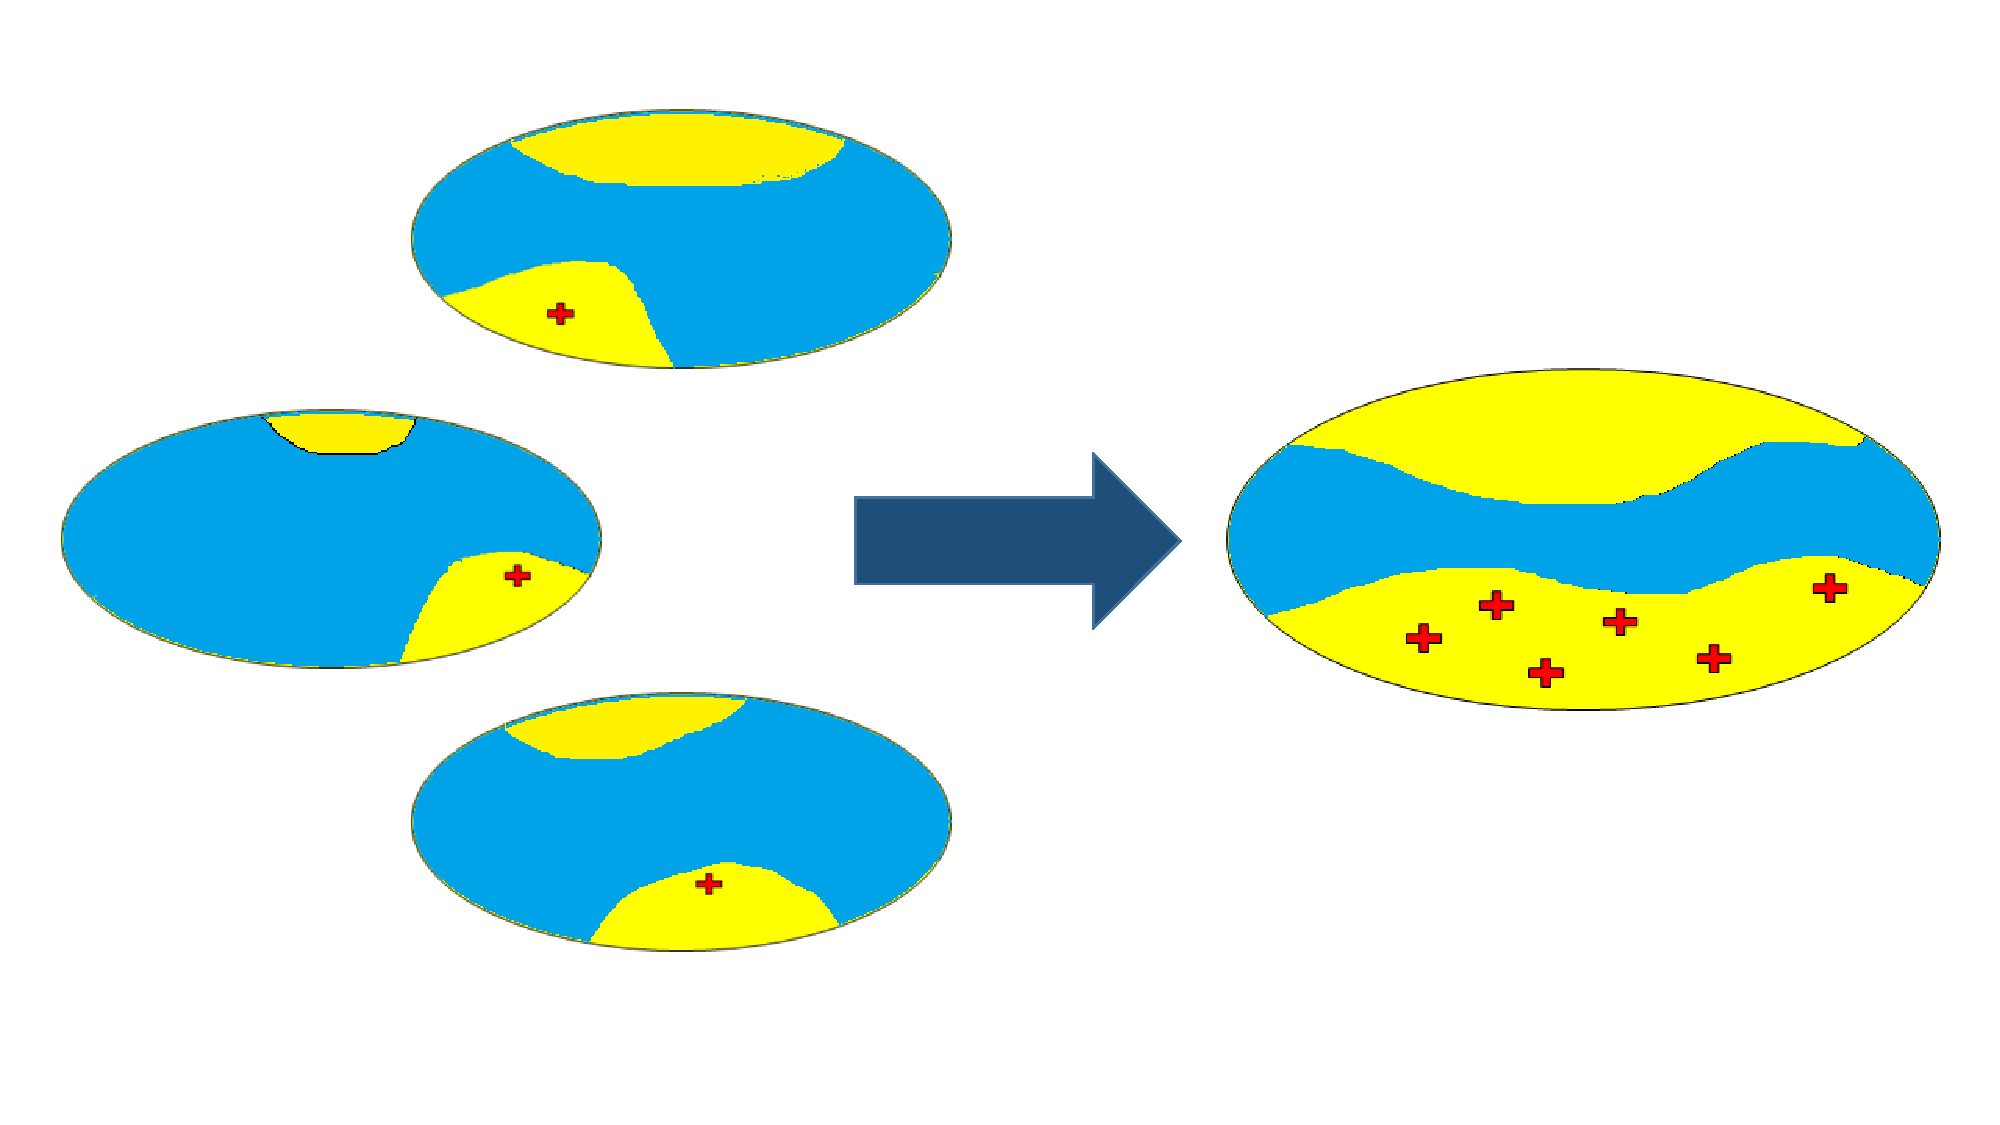
\includegraphics[width=0.9\columnwidth]{figures/argument_generalization}
%	\caption{Argument Generalization.}
%	\label{fig:argument_generalization}
%\end{figure}

%\begin{equation}
%\label{relation_saliency}
%RS_{ij}=\frac{Count(rel_i,R_j)}{Count(R_j)}
%\end{equation}
%pick $rel_i$ for $R_j$ as relation constraint, where $i=argmax_i RS_{ij}$
%	\subsubsection{Rule Subsuming.}
%	after we put the rule into the rule base, if the frequency of this rule reach a threshold, the system will trigger the rule subsuming function, which will generalize this rule together with previous rule to get a more general rule.
%		\begin{algorithm}[htb]
%		\caption{Online Causality Rule Learner.\label{alg:oclr}} 
%		\KwIn{ free text} 
%		\KwOut{First-order logic Rules}
%		rule instances extractions
%		generalize all the rule instances' predicates.\\
%		\For{ rule instances set I with the same predicate}{
%		R=Rule\_Induction(I)\\
%		add the relation constraints for these rules
%		}
%	\end{algorithm}	
\noindent
\textbf{Rule Confidence}
Knowledge discovered from noisy data is uncertain. Therefore, we combine the following features of the learned rules to give each rule a confidence value. For a given rule, we consider:
the frequency of the predicate pair in cause event and effect event,
the number of rule instances that generalizes to this rule,
the pattern priority of the rule instances extracted from the sentences,
and the frequency of event roles in this rule.
Then, get the numeric values of these features of all rules and normalize them to a range of 0 to 1. Finally, the weighted sum is calculated as rule confidence, where the corresponding weight is (0.5, 0.2, -0.1, 0.5).
\begin{figure}[htbp]
	\centering
	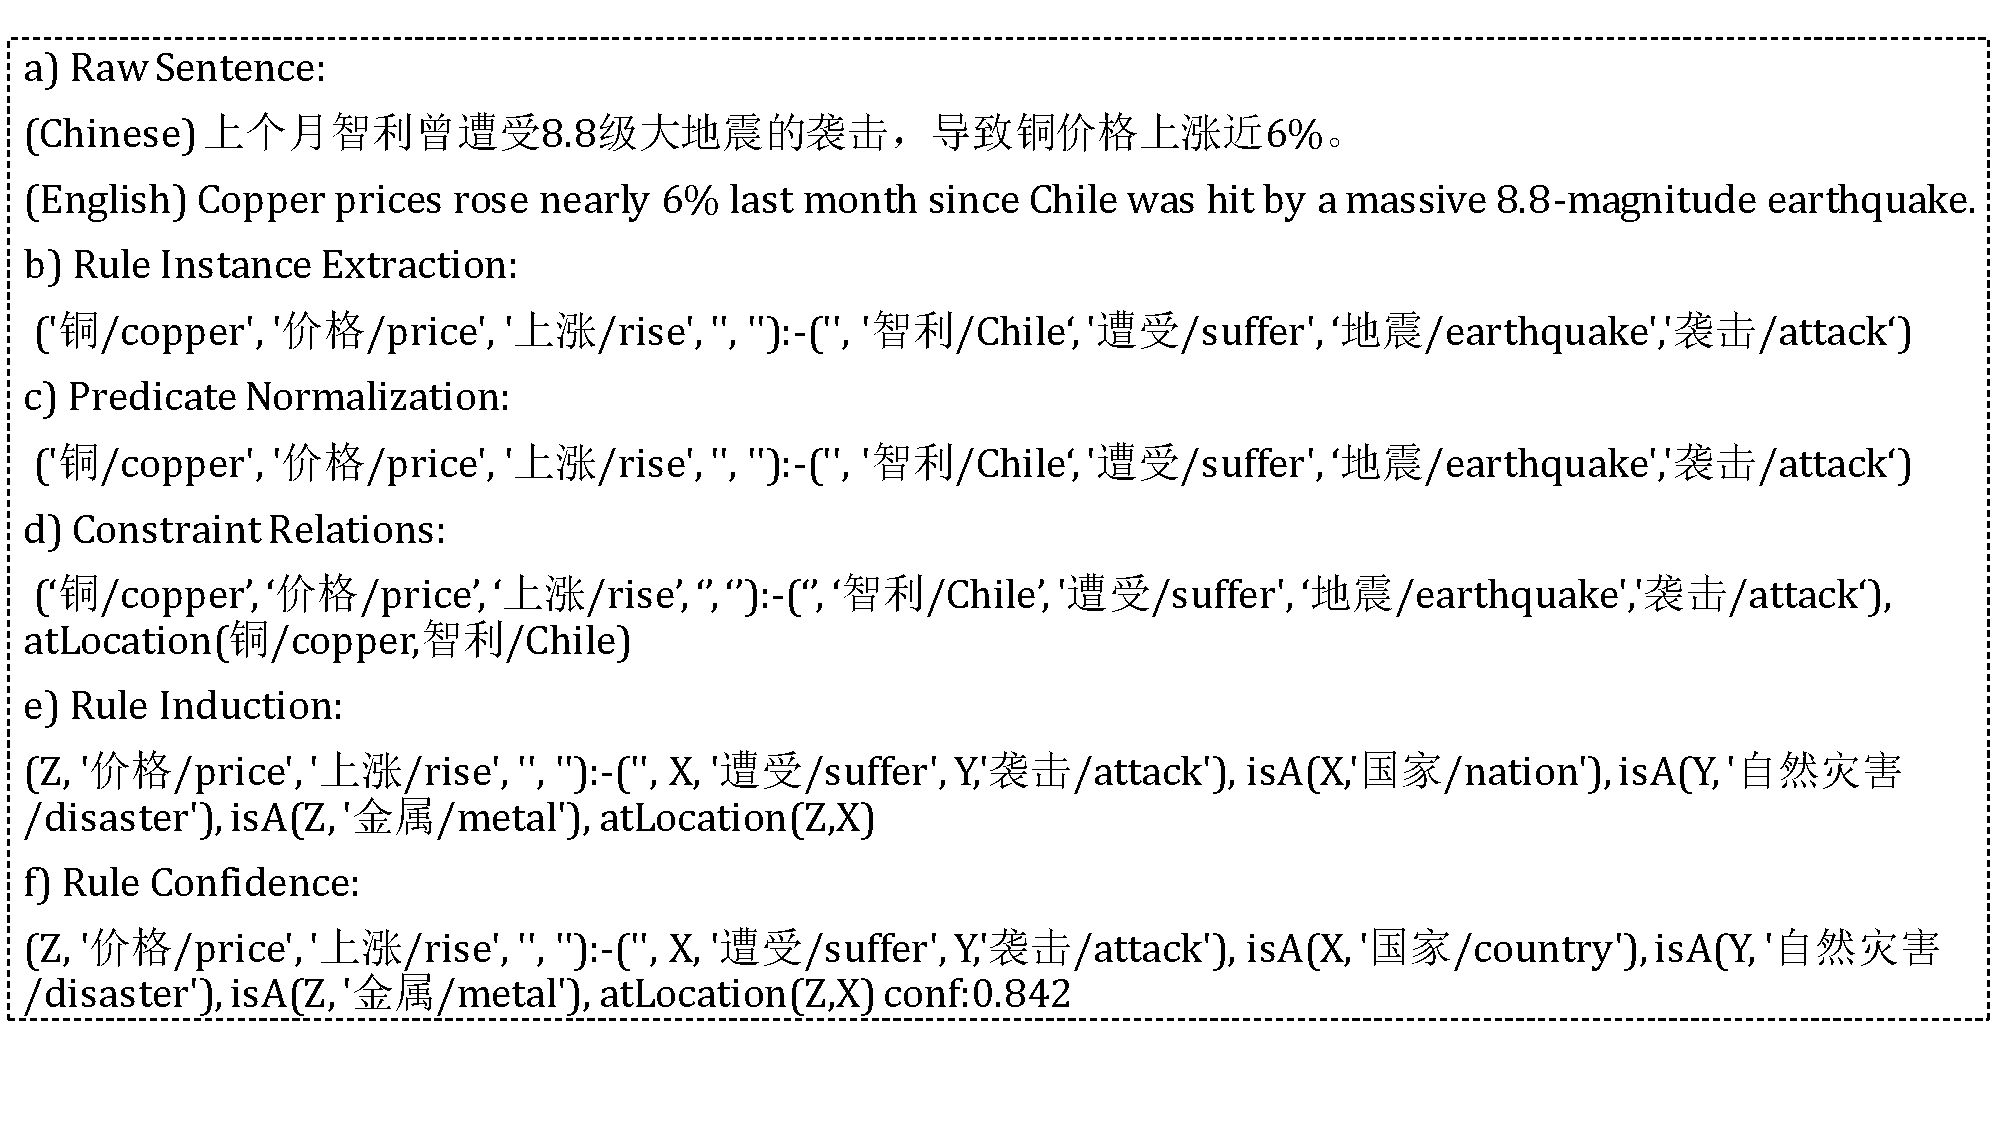
\includegraphics[width=0.95\columnwidth]{figures/example}
	\caption{An Example Showing Various Stages of the Framework}
	\label{fig:stages_in_an_example}
\end{figure}

\subsection{Causal Reasoning}
The specific reasoning process is as follows. Extract the query event from a given query sentence, search related rules in the learned rules with the depth-first search algorithm, look up related facts in Probase and ConceptNet to reduce the size of the facts and rules to speed up reasoning, and convert the found rules and facts into Prolog code together. 
To implement uncertain reasoning, we put rule confidence into the generated Prolog code and 
%use multiplication to decline the confidence in reasoning.
use multiplication to simulate the decline of the confidence in reasoning.
Uncertain reasoning should reduce confidence as reasoning deepens. We set the threshold $\gamma$ to cut off more in-depth reasoning. 
%We choose Prolog for reasoning with uncertainty because it is a mature and reliable tool, instead of ProbLog \cite{de2007problog} and PSL \cite{bach:jmlr17}.
Small modification of Prolog code generalization is enough to reason with uncertainty, so we choose the mature and reliable Prolog, instead of ProbLog \cite{de2007problog} and PSL \cite{bach:jmlr17}.
After generating the Prolog code, we query the query event in the Prolog code format and finally return the top K results sorted by the confidence.